%%%%%%%%%%%%%%%%%%%%%%%%%%%%%%%%%%%%%%%%%
% Wenneker Assignment
% LaTeX Template
% Version 2.0 (12/1/2019)
%
% This template originates from:
% http://www.LaTeXTemplates.com
%
% Authors:
% Vel (vel@LaTeXTemplates.com)
% Frits Wenneker
%
% License:
% CC BY-NC-SA 3.0 (http://creativecommons.org/licenses/by-nc-sa/3.0/)
% 
%%%%%%%%%%%%%%%%%%%%%%%%%%%%%%%%%%%%%%%%%

%----------------------------------------------------------------------------------------
%	PACKAGES AND OTHER DOCUMENT CONFIGURATIONS
%----------------------------------------------------------------------------------------

\documentclass[11pt]{scrartcl} % Font size

%%%%%%%%%%%%%%%%%%%%%%%%%%%%%%%%%%%%%%%%%
% Wenneker Assignment
% Structure Specification File
% Version 2.0 (12/1/2019)
%
% This template originates from:
% http://www.LaTeXTemplates.com
%
% Authors:
% Vel (vel@LaTeXTemplates.com)
% Frits Wenneker
%
% License:
% CC BY-NC-SA 3.0 (http://creativecommons.org/licenses/by-nc-sa/3.0/)
% 
%%%%%%%%%%%%%%%%%%%%%%%%%%%%%%%%%%%%%%%%%

%----------------------------------------------------------------------------------------
%	PACKAGES AND OTHER DOCUMENT CONFIGURATIONS
%----------------------------------------------------------------------------------------

\usepackage{amsmath, amsfonts, amsthm} % Math packages

\usepackage{listings} % Code listings, with syntax highlighting
\usepackage[outputdir=out]{minted}

\usepackage[english]{babel} % English language hyphenation

\usepackage{graphicx} % Required for inserting images
\graphicspath{{Figures/}{./}} % Specifies where to look for included images (trailing slash required)

\usepackage{booktabs} % Required for better horizontal rules in tables

\numberwithin{equation}{section} % Number equations within sections (i.e. 1.1, 1.2, 2.1, 2.2 instead of 1, 2, 3, 4)
\numberwithin{figure}{section} % Number figures within sections (i.e. 1.1, 1.2, 2.1, 2.2 instead of 1, 2, 3, 4)
\numberwithin{table}{section} % Number tables within sections (i.e. 1.1, 1.2, 2.1, 2.2 instead of 1, 2, 3, 4)

\setlength\parindent{0pt} % Removes all indentation from paragraphs

\usepackage{enumitem} % Required for list customisation
\setlist{noitemsep} % No spacing between list items

%----------------------------------------------------------------------------------------
%	DOCUMENT MARGINS
%----------------------------------------------------------------------------------------

\usepackage{geometry} % Required for adjusting page dimensions and margins

\geometry{
	paper=a4paper, % Paper size, change to letterpaper for US letter size
	top=2.5cm, % Top margin
	bottom=3cm, % Bottom margin
	left=3cm, % Left margin
	right=3cm, % Right margin
	headheight=0.75cm, % Header height
	footskip=1.5cm, % Space from the bottom margin to the baseline of the footer
	headsep=0.75cm, % Space from the top margin to the baseline of the header
	%showframe, % Uncomment to show how the type block is set on the page
}

%----------------------------------------------------------------------------------------
%	FONTS
%----------------------------------------------------------------------------------------

\usepackage[utf8]{inputenc} % Required for inputting international characters
\usepackage[T1]{fontenc} % Use 8-bit encoding

\usepackage{fourier} % Use the Adobe Utopia font for the document

%----------------------------------------------------------------------------------------
%	SECTION TITLES
%----------------------------------------------------------------------------------------

\usepackage{sectsty} % Allows customising section commands

\sectionfont{\vspace{6pt}\centering\normalfont\scshape} % \section{} styling
\subsectionfont{\normalfont\bfseries} % \subsection{} styling
\subsubsectionfont{\normalfont\itshape} % \subsubsection{} styling
\paragraphfont{\normalfont\scshape} % \paragraph{} styling

%----------------------------------------------------------------------------------------
%	HEADERS AND FOOTERS
%----------------------------------------------------------------------------------------

\usepackage{scrlayer-scrpage} % Required for customising headers and footers

\ohead*{} % Right header
\ihead*{} % Left header
\chead*{} % Centre header

\ofoot*{} % Right footer
\ifoot*{} % Left footer
\cfoot*{\pagemark} % Centre footer
 % Include the file specifying the document structure and custom commands

%----------------------------------------------------------------------------------------
%	TITLE SECTION
%----------------------------------------------------------------------------------------

\title{	
	\normalfont\normalsize
	\textsc{SZ-Ybbs}\\ % Your university, school and/or department name(s)
	\vspace{25pt} % Whitespace
	\rule{\linewidth}{0.5pt}\\ % Thin top horizontal rule
	\vspace{20pt} % Whitespace
	{\huge Proxmox vs vSphere}\\ % The assignment title
	\vspace{12pt} % Whitespace
	\rule{\linewidth}{2pt}\\ % Thick bottom horizontal rule
	\vspace{12pt} % Whitespace
}

\author{\LARGE Erber Jakob \and \LARGE Freunberger Raphael} % Your name

\date{\normalsize\today} % Today's date (\today) or a custom date

\begin{document}

\maketitle % Print the title

\section{Introduction}

\section{Introduction}
This document will compare the two hypervisors Proxmox and vSphere.
\\\\
Proxmox is an open-source hypervisor based on Debian. Proxmox is mostly used for home labs or small businesses. It is free to use, but you can buy a subscription to get support.
\\\\
vSphere is a proprietary hypervisor developed by VMWare. It is used in enterprise environments and is only available for a fee.

\subsection{Understanding vSphere}

vSphere has a lot of different components, with different names. Understanding the naming of some of them will be crucial for the rest of the document.
\\\\
\begin{itemize}
	\item vSphere: The entire virtualization platform
	\item ESXi: The hypervisor running on the physical hardware
	\item vCenter: The service for managing multiple ESXi hosts
\end{itemize}

\subsection{Installation}

We tried to install both hypervisors to test them and make images for this document, but we ran into issues with vSphere.
\\\\
Both the ESXi 7.0 and 8.0 ISOs provided by out teacher did not run under Hyper-V, always getting stuck on ``Relocating modules and starting up the kernel''.

With KVM the installation worked, but we were not able to connect to the web interface, because of some problem with ESXi and the virtualized network interface.

Finally the VMWare Workstation VM provided by our teacher did work, however VMWare Workstation needs you to disable Hyper-V and memory integrity on a Windows 11 host to use nested virtualization. Since we use Hyper-V for Proxmox and turning off memory integrity is a security risk we chose not to do this. Without nested virtualization we were not able to run a VM inside ESXi.

\section{Requirements}

Since Proxmox focuses on smaller environments with weaker hardware the hardware requirements to run Proxmox are very low. Pretty much any AMD or Intel system manufactured within the last 10 years should meet the requirements.

\begin{itemize}
	\item x86-64 CPU with VT/AMD-V enabled
	\item 2GB memory
	\item About 16GB disk space for the hypervisors OS
\end{itemize}

\subsection{vSphere}
For vSphere the requirements are higher and only Intel Xeon, AMD Epyc and some specific SKUs of the intel core series are officially supported. 
If you try to install ESXi v8 on an unsupported CPU you will get a warning and can only choose to reboot the system. There is a workaround with a kernel flag, but you will almost certainly not get any support from VMWare if you do so. 

\begin{itemize}
	\item x86-64 CPU with at least 2 cores with VT/AMD-V enabled
	\item 8GB memory
	\item 32GB boot disk
\end{itemize}

\section{Snapshots}

\section{Snapshots}

A snapshot stores the state of a virtual machine at a specific point in time. This allows you to revert to that state, should you need to. Unlike backups which store the entire state of the virtual machine, snapshots only store the changes made since the snapshot was taken.
\\\\
The snapshot feature is very similar in Proxmox and vSphere. Both support making extensive snapshot trees, where you can have snapshots of a snapshot of a snapshot including different branches. You can choose whether to also snapshot the memory state of the VM or not. In Proxmox the VM disk must either be stored as qcow2 image available to file level storage, or on a storage type that supports snapshots. For a complete list see~\ref{tab:storageTable}.
\\\\
Here is an example of a snapshot tree in Proxmox, the VM is currently running under the state of test1, but I could always revert back to test2 through test4.

\begin{figure}[H]
	\centering
	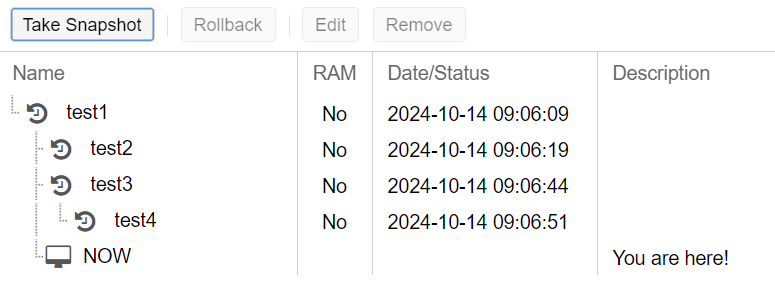
\includegraphics[width=0.8\linewidth]{Proxmox_snapshots.png} % Figure image
	\caption{Snapshot tree in Proxmox} % Figure caption
	\label{fig:Snapshot tree in Proxmox} % Label for referencing with \ref{bear}
\end{figure}

\section{Migration}

\subsection{Live Migration}
\subsection{Convert between different hypervisors}

\section{Datastores}

\section{HA}

\section{Management}


\section{Licensing}

\subsection{Comparison}

\paragraph{Proxmox} 
is \textbf{open-source} and offers all features for free by default for private and/or commercial use. Aditionally, Proxmox offers 4 simple subscription-based models for enterprises which offer technical support and access to the \enquote{Proxmox Enterprise Repository}, which provides reliable updates and security patches. The available subscription models are:
\begin{itemize}
	\item \textbf{Community}:\num{ 110}€/year \& CPU-Socket
	\item \textbf{Basic} \num{340}€/year \& CPU-Socket
	\item \textbf{Standard} \num{510}€/year \& CPU-Socket
	\item \textbf{Premium} \num{1020}€/year \& CPU-Socket
\end{itemize}
All of them offer access to the enterprise repository but they differ in the quality and quantity of their technical support.\newline
An example setup consisting of 3 hosts and a 32-core CPU each will cost from \num{330}€/year to \num{3060}€/year depending on the amount of support wanted. (or nothing on the free edition)


% https://community.veeam.com/blogs-and-podcasts-57/decoding-the-new-broadcom-vmware-vsphere-licensing-packages-for-small-deployments-6398
\paragraph{VMware} requires more complex licensing.\newline
ESXi hosts are licensed with vSphere licenses. There is one main license model and a few older models which are no longer sold but are still supported. The current licensing model is per core licensing with a minimum of 16 cores per CPU. All licenses are sold in different editions:\newline 
\textit{The following prices are based on the MSRP when using a 3-year subscription. VMware offers 1, 3 and 5 year subscriptions with varying prices.}

\subparagraph{vSphere Essentials Plus Kit}
is sold in 96 core license packs and includes vCenter Essentials for up to 3 hosts with a price of \num{35}\$/core/year which totals to \num{3360}\$/year or \num{10080}\$/3-years.

\subparagraph{vSphere Standard} includes vCenter Server Standard and is priced at \num{50}\$/core/year. It does not have a upper limit on hosts or cores. A license with 96 cores would cost \num{14400}\$/3-years 

\subparagraph{vSphere Foundation} includes vSphere Enterprise Plus, vCenter Server Standard, Tanzu Kubernetes Grid, Aria Suite Standard and available Add-On's. Additionally it includes 100GiB of vSAN Enterprise per-core. The price is \num{135}\$/core/year. 
A license with 96 cores would cost \num{38880}\$/3-years.


\subparagraph{Other models,} which are no longer being sold, include: 
\begin{itemize}
	\item per-CPU licensing with a maximum of 32 cores per license. For CPUs with more than 32 cores multiple licenses have to be acquired
	\item pre-VM licensing
	\item vSphere+ capacity based licensing
\end{itemize}

\subparagraph{Evaluation} is possible with a 60-day trial license.
It starts as a free 60-day trial and can be converted to a full license by purchasing a license key. The license key is entered into the vSphere Client and the evaluation license is converted to a full license.

\subsection{Conclusion}

Proxmox's licensing solely provides additional support and updates, while the software itself is free and open-source. 
VMware is proprietary and not free. The licensing is more complex and expensive, but it offers more features and support. 


\end{document}
